\section{Method}

\subsection{Task Formulation}

\hspace{1pc}We use imitation learning (IL) to train the proposed BID.
In IL, expert first demonstrates a driving action $a_{t}$ (such as steering, brake and throttle) in response to an input frame $f_t$ based on the expert's policy $\pi(f_{t})$.
It reflects the expert's driving skills, judgement, and behavior.
The core idea of IL is to train the proposed BID agent to replicate the expert's actions by learning from these observed interactions.

\begin{figure*}[t]
	\centering
	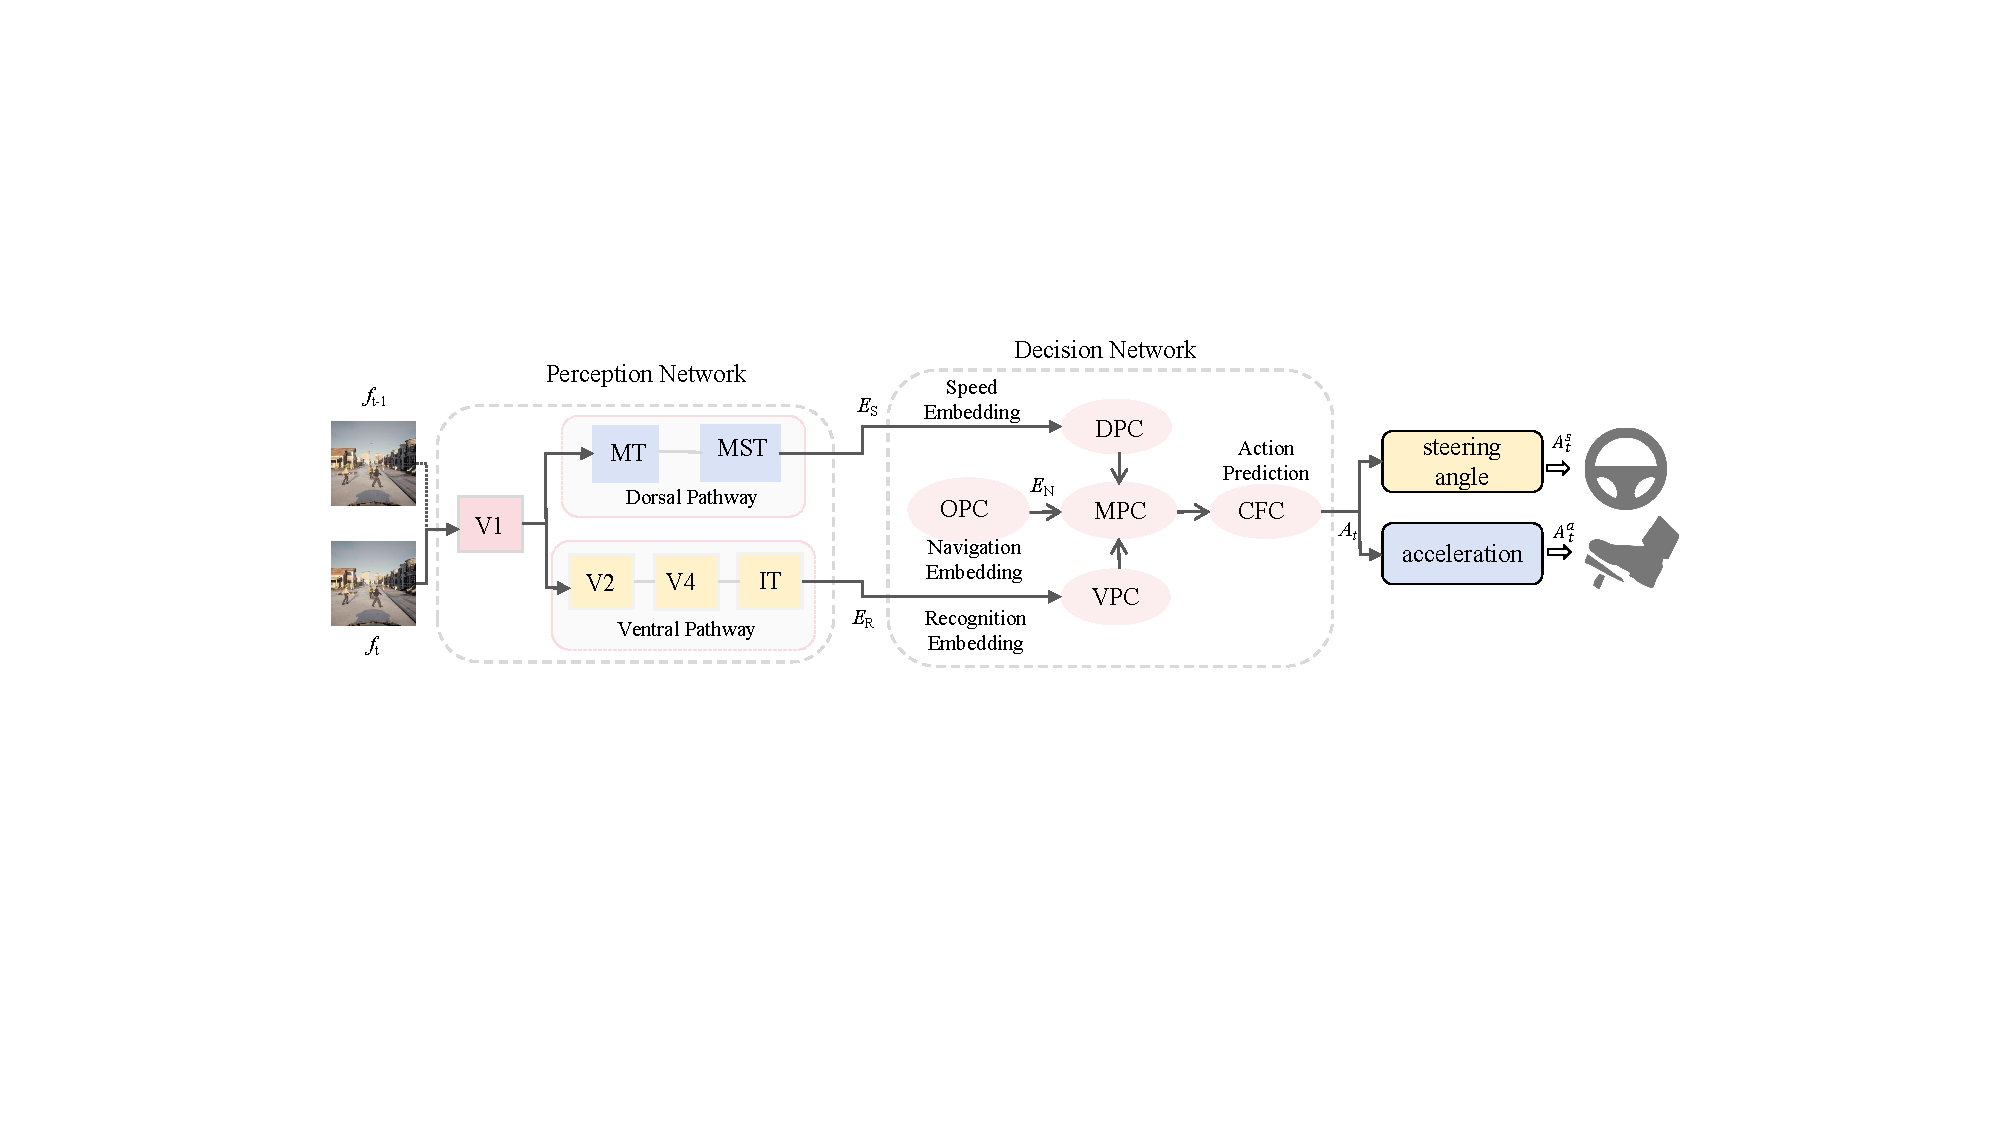
\includegraphics[width=\linewidth]{fig/net.pdf}
	\caption{The network architecture of the BID agent is primarily composed of the perception network and the decision network.
		The perception module includes both the dorsal and ventral pathways, which allow the system to understand and process its surroundings.
		The decision network consists of five modules that represent different regions of the prefrontal cortex: the medial prefrontal cortex (MPC), orbital prefrontal cortex (OPC), caudal prefrontal cortex (CPC), dorsal prefrontal cortex (DPC), and ventral prefrontal cortex (VPC). 
		Specifically, the input to the system is an RGB image $f_{t} $, which represents the current visual scene.
		The output is the action $A_t$, which controls the ego-vehicle's maneuvering directly.
		The action $A_t$ includes the steering angle $ A_t^s $ and acceleration $ A_t^a $ of the vehicle, making BID a brain-inspired and end to end autonomous driving model.
		Besides, in the construction process of training dataset, the driving actions and input frames are paired.
	}
	\label{fig:fig2}
\end{figure*}

Before training the BID using IL, we first collect a series of frame and action pairs $(f_{t}, a_{t})$ produced by expert demonstrations.
These data are then utilized to train the BID policy $\pi_{\theta}(f_{t})$, which approximates the expert's policy.
%The overall objective of imitation is 
%\begin{equation} \label{eq:target}
%	\argmin_{\theta} \mathbb{E}_{(\mathbf{f}_{i}, \mathbf{a}_{i})\sim \mathcal{D}} \left[ \mathcal{L}(\pi_{\theta}(\mathbf{f}_{i}), \mathbf{a}_{i}) \right] \enspace .
%\end{equation}
%
In the validating phase, we no longer utilize the expert's strategy, but only the trained BID policy.




\subsection{Neural Aligned BID}
\hspace{1pc}Inspired by the brain's remarkable capabilities in perception and decision-making, we have proposed the perception and decision network based on neural pathway anatomical alignment to simulate the information processing mechanisms of brain in an autonomous driving system. 
This approach is designed to significantly improve both the interpretability and robustness of the system.

\subsubsection{Perception Network}
\hspace{1pc}As shown in Fig.~\ref{fig:fig2}, our brain-inspired perception network begins by capturing precise input data from the surrounding environment, which includes essential traffic elements such as roads, vehicles, pedestrians, and traffic signals. 
% 模型的输入
% the ego vehicle's forward speed $s_t\in\mathbb{R}$
% data $f_t$ consists of 3 horizontally continuous frames from camera.
% s $f_{t}=\{f_{t,1}, f_{t,2}, f_{t,3} \}$
At time $t$, the input frame $f_t$ is processed through a series of deep convolutional neural networks and recurrent networks, incorporating activation functions commonly used in deep neural networks. 
This processing mirrors the way external information is handled by the brain's visual cortex\cite{kubilius2019brain}. 
Initially, the primary visual cortex (V1) processes the visual input, extracting key features. 
To manage the high computational demands, the first area, V1$_\text{BID}$, includes a 7$\times$7 convolution operation and another 3$\times$3 convolution. 
% with stride 2, a 3$\times$3 pooling operation with stride 2,
These features are then passed along to the dorsal visual pathway, where middle temporal (MT) and middle superior temporal (MST) specialize in encoding velocity information between current frame $ f_t $ and previous frame $ f_{t-1} $, particularly related to spatial location and movement\cite{wang2022btn}. 
The dorsal pathway is implemented as a dynamic filter network\cite{jia2016dynamic} and utilized to extract the spatial relation between background and foreground, 
and uses appearance repsentation $ \alpha_t $ to dynamically infer convolutional filter.


% 腹侧
At the same time, the ventral pathway receives these features, with inferior temporal (IT) cortex focusing on encoding object category information, thereby facilitating object recognition.
% Cornet
Each visual area in ventral pathway is simulated with a specific module, where neurons perform some classical, standard operations, such as convolution, nonlinearity, batch normalization, and max pooling on its input. 
The structure of the pathway is same across all visual areas, though the number of cells for a submodule may vary.
The subsequent areas, V2$_\text{BID}$, V4$_\text{BID}$ and IT$_\text{BID}$, each carry out two 1$\times$1 convolutional opeartion, a 3 $ \times $ 3 bottleneck style convolutional operation, and another 1$\times$1 convolution. 
To simulate recurrent connection, the output for each submodule are fed back into the same submodule 4 times for further processing.


%
After this sequence of processing steps, our network is capable of efficiently extracting and outputting multi-dimensional embeddings of the current environment to next decision network. 
These features include both the appearance characteristics $ E_V $ of objects and motion-related information $ E_S $.



\subsubsection{Decision Network}
% 决策模块
The output features from the perception network are then efficiently passed to a brain-inspired decision-making network, where they undergo further processing through transformer networks, along with anatomical alignment to the prefrontal cortex pathway. 
This simulates how sensory information is processed by different regions of the prefrontal cortex in the brain.
%


% 腹侧
The ventral prefrontal cortex (VPC) generates goals based on recognition embedding (visual cues), allowing for quick responses and adaptation to changes in the environment\cite{passingham2012neurobiology}.
%
In our setup, we flatten the embedding patches and then fed it to transformer models.
We use the classical one-dimensional position feature~\cite{Alexey:2021} to offer positional context, and add this embedding directly to the token.


% 背侧
The dorsal prefrontal cortex (DPC) is responsible for generating goals based on sequences, as well as temporal and spatial environmental cues, offering clear guidance for decision-making and action\cite{passingham2012neurobiology}.
DPC is implemented with a dynamic filter network~\cite{jia2016dynamic} and is used to address spatial relations between the foreground and background.
% 眶额
Within this process, the orbitofrontal cortex (OFC) plays a crucial role in establishing future action goals $n_t$, which is encoded as a one-hot command embedding.
It helps to clarify and focus on the desired objectives. 
% 速度、导航命令
The navigation command $n_t$ is mapped into a vector embedding $E_N$ using a fully connected layer (FC).
% and forward speed $s_t$



% 内侧
The medial prefrontal cortex (MPC) is critical for making decisions based on current states, along with a high-level navigation command\cite{passingham2012neurobiology}.
It ensure that our actions are optimized according to previous experiences and future goal.
The input embeddings of MPC are merged with the output of VPC, DPC and OFC.
We format the BID with the input data $O_t=(f_t, n_t)$, parameterized by $ \pi_{\theta}(f_t, n_t) $, as
\begin{equation}\label{eq:encoder}
	A_t^s, A_t^s = \pi_\text{MPC}(E_S, E_N, E_V).
%	e_{\theta}: \mathbb{R}^{|\mathbf{X}_{t}|\times W\times H\times3}\times\mathbb{R}\times \mathbb{R}^k \rightarrow \mathbb{R}^{S \times c} \enspace .
\end{equation}


Navigation embedding $E_{t}$ is used as a switch to activate various multilayer perceptron branches for inferring $A_{t}$ in CIL \cite{Codevilla:2018} and LBC~\cite{Codevilla:2019}. 
However, in our approach, we use a transformer to process the positional embedding $ E_V $.
To simplify the learning process, we utilize the navigation command $n_{t}$ as additional inputs.
%
% 注意力学习
% 连接3个图像
We leverage the self-attention method in transformer to effectively extract multi-view feature\cite{Vaswani:2017}.
This approach allows the model to extract the relationships among remote frame patches, enabling it to link representation for horizontal perspectives of vehicle.


% CFC
In MPC, a traffic representation is learned utilizing the transformer module with multiheaded self-attention layer~\cite{Vaswani:2017}, normalization~\cite{Ba:2016}, and feed forward multilayer perceptron modules. 
% 尾侧
The caudal prefrontal cortex (CPC) is crucial for searching, identifying, and locating specific targets, ensuring that we can accurately focus on and navigate towards these targets\cite{lawler1987role}. 
% 总结
These regions work together in the decision-making process, forming a highly integrated latent feature vector that effectively captures the essential information needed for making decisions\cite{wardak2004deficit}. 
This latent vector is then processed through a carefully constructed hidden layer, which generates accurate and reliable outputs, such as driving actions, value function estimates, and speed control commands.
The final output is obtained by linearly projecting the merged features for a self-attention head, which are passed to the CPC module.
We utilize 4 layers, and a layer with 4 attention modules. 
The middle size in the transformer module is matched with the output size of the ResNet.
%
% 动作预测
The output from the transformer encoder is average pooled and passed through a multilayer perceptron.
This multilayer perceptron includes 3 FC with nonlinearity between layers.
The driving hehavior $A_t$ represents the vehicle acceleration $A_t^s$ (throttle and brake) and the wheel angle $A_t^s$ as depicted in Equ.~\ref{eq:encoder}. 





\subsection{Loss Function}

\hspace{1pc}The BID network is designed to replicate the advanced information processing abilities of the human brain by carefully aligning neural pathways with corresponding network modules. 
Through iterative updates, the network adjusts its parameters to better match human decision-making processes, ultimately improving its performance and accuracy.
%
% 损失函数
Based on the inferred output $A_t$ and the expert's actual output $\hat{A}_t$, the model loss function is described as:
\begin{equation}\label{eq:loss}
	L(A_t, \hat{A}_t) 
	= \lambda_{s} \lVert A_{t}^s-\hat{A}_t^s \rVert_{1}
	+ \lambda_{a}\lVert A_{t}^a-\hat{A}_{t}^a\rVert_{1} \enspace ,
\end{equation}
where $\lambda_{s}$ and $\lambda_a$ represent the steering angle and vehicle acceleration loss weight.
$\lVert\cdot\rVert_{1}$ denotes the Manhattan distance.
The weights are set as $\lambda_{s} = \lambda_{a} = 0.5$. 
Both vehicle acceleration and wheel angle are constrained within the range of $[-1, 1]$.
A acceleration greater than zero denotes throttle and a acceleration less than zero indicates braking in these work.


In behavior cloning~\cite{Codevilla:2019}, they use velocity inference regularization incorporated into the loss function to address the inertial issue resulting from the high likelihood of the ego vehicle remaining stationary.
However, we did not encounter this issue, and therefore, the velocity inference module is not included in the proposed BID model.
It is sufficient to achieve a excellent driving result with a plain training loss depicted in Equ.~\ref{eq:loss}, even in unfamiliar environments.
%
%Additionally, the outputs from both the brain-inspired perception network and the brain-inspired decision network are concatenated to form a latent feature that captures critical driving-related information. 
%This latent feature is then passed through a hidden layer to map it to driving actions.


%\subsubsection{Brain-Expert Mimetic Entity}
%
%\hspace{1pc}\textbf{\textsf{Agent.}} The BID agent utilizes imitation learning to predict driving behavior based on the current state, supervised by extensive data generated by the reinforcement learning expert. The structure of the agent is illustrated in Fig. \ref{fig:fig2}.

%\textbf{\textsf{Loss Function.}} 
%In the decision-making stage, for each command, a branch is constructed. 
%All branches share the same architecture, with each branch containing an action head for predicting the continuous action $\mathbf{a}$ and a velocity head for predicting the current vehicle speed $\mathbf{s}$. 
%And $\mathbf{\hat{a}}$ represents the expert's action,$\mathbf{\hat{s}}$ is the measured speed, and $\mathbf{a}$ and $\mathbf{s}$ are the actions and speeds predicted by the agent, respectively. 
%\begin{align}
%   \mathcal{L} = \|\hat{\mathbf{a}}-\mathbf{a}\|_{1}^{2} + \lambda_{\mathrm{S}} \cdot (\hat{s}-s)^{2} + \lambda_{\mathrm{F}} \cdot \left\| \mathbf{j}_{\mathrm{NR}}-\mathbf{j}_{\mathrm{BID}} \right\|_{2}^{2}
%\end{align}


\begin{comment}
\subsection{Similarity Metrics}
\hspace{1pc}\textbf{\textsf{Collecting Brain Activation Signals.}} To align the network, we collect the brain's responses to multi-channel grayscale images. Initially, EEG sensors are placed at appropriate locations and connected to data acquisition equipment. Subsequently, neuroimaging software is utilized to preprocess cortical activation data. Then, the brain data is aligned with standard data to ensure consistency, followed by noise removal and data smoothing. Ultimately, we obtain activation signals from visual brain regions that vary over time as participants view different images. These signals are further amplified through deconvolution processing to reveal the brain's activation patterns.

\textbf{\textsf{Network Alignment.}} To achieve a closer alignment with human brain functions, the network parameters are continuously optimized, thereby significantly enhancing the bionic performance and simulation accuracy of the network.


% 性能度量标准
\textbf{\textsf{Metrics:}}
Our results are reported in success rate, the metric proposed by NoCrash, and driving score, a new metric introduced by the CARLA LeaderBoard. 
The success rate is the percentage of routes completed without collision or blockage. 
The driving score is defined as the product of route completion, the percentage of route distance completed, and infraction penalty, a discount factor that aggregates all triggered infractions.
For example, if the agent ran two red lights in one route and the penalty coefficient for running one red light was $0.7$, then the infraction penalty would be  $0.7^{2}$$=$$0.49$.
Compared to the success rate, the driving score is a fine-grained metric that considers more kinds of infractions and it is better suited to evaluate long-distance routes.
More details about the benchmarks and the complete results are found in the supplement.


\textbf{\textsf{Similarity Assessment.}} After parameter tuning, the BID network is capable of simulating the mechanisms of the human brain in environmental recognition and decision-making. Following each optimization, we accurately calculate the similarity between the BID and the human brain. The degree of congruency between the brain-inspired network and the human brain is quantified by computing the average of activation similarity and decision similarity through the specified formula. Notably, $S_{X_{p}}$ and $S_{X_{d}}$ denote the standard deviations of the model's activation sample points and decision sample points, respectively, whereas $S_{Y}$ represents the corresponding data values of the human brain.
\begin{align}
	r & = \frac{1}{2}\left(\frac{Cov_{X_{p},Y_{p}}}{\sqrt{S_{X_{p}} S_{Y_{p}}}}+\frac{Cov_{X_{d},Y_{d}}}{\sqrt{S_{X_{d}} S_{Y_{d}}}}\right)
\end{align}
%\begin{align}
%	r & = \frac{1}{2}\left(\frac{\sum_{i = 1}^{n}\left(X_{p_{i}}-\bar{X_{p}}\right)\left(Y_{p_{i}}-\bar{Y_{p}}\right)}{\sqrt{\sum_{i = 1}^{n}\left(X_{p_{i}}-\bar{X_{p}}\right)^{2}} \sqrt{\sum_{i = 1}^{n}\left(Y_{p_{i}}-\bar{Y_{p}}\right)^{2}}} \right. \nonumber \\
%	& \qquad \left. + \frac{\sum_{i = 1}^{n}\left(X_{d_{i}}-\bar{X_{d}}\right)\left(Y_{d_{i}}-\bar{Y_{d}}\right)}{\sqrt{\sum_{i = 1}^{n}\left(X_{d_{i}}-\bar{X_{d}}\right)^{2}} \sqrt{\sum_{i = 1}^{n}\left(Y_{d_{i}}-\bar{Y_{d}}\right)^{2}}} \right)
%\end{align}

\end{comment}